\section{Introduction}

Post-quantum cryptography is moving from a standards problem to a systems problem.  Once secure services adopt ML-KEM, ML-DSA, and related post-quantum mechanisms, the write path of a TLS terminator, key-management service, or signed logging system begins to carry more than application payload.  It also carries KEM ciphertexts, encapsulation metadata, session secrets, key-wrap records, certificate metadata, and signatures.  These objects are not all alike: some are append-only audit records, some are public metadata, and some are short-lived secrets whose lifetime ends at session close, epoch advance, or key rotation.

Zoned Namespace SSDs are a natural substrate for such services because they expose the structure that log-structured systems already exploit: data is appended into zones and reclaimed by resetting whole zones.  The placement problem is therefore crucial.  If objects that die together are placed together, a zone reset can reclaim space with little or no valid-block copying.  If short-lived and long-lived objects are mixed, the host must either copy residual live blocks during GC or leave expired data in place until a future cleaner selects the zone.  Recent \zns and log-structured placement systems, including \sepbit, \midas, and \dogi, attack this problem by inferring block lifetime from storage-visible history such as LBA, frequency, age, segment behavior, and prior invalidation time~\cite{sepbit,midas,dogi}.

The central mismatch in post-quantum workloads is that the lifetime of cryptographic artifacts is often not hidden at all.  The application or cryptographic runtime already knows that a session secret will die at session close, that a KMS envelope belongs to an epoch, and that a certificate object follows a rotation policy.  The storage device does not see this state.  From the perspective of a history-based placement system, a KEM artifact may look like another small write near a hot payload record.  From the perspective of the protocol, it belongs to a death cohort: a set of objects that become invalid together when the cryptographic state advances.

\begin{figure*}[t]
\centering
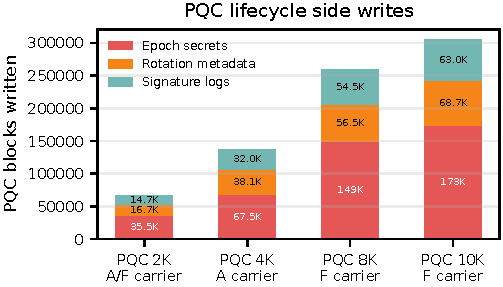
\includegraphics[width=0.68\textwidth]{../artifacts/figures/fast-style/fig1-intro-pressure.pdf}
\caption{Actual-\zns YCSB pressure with all history-based baselines.  The low-pressure row is intentionally a negative WAF control, while higher PQC overlays create GC pressure.  FIFO, \sepbit-style, \midas-style, and \dogi-style placement all leave expired secret blocks because they cannot see protocol death cohorts; \system-\dogi keeps secret cohorts reset-eligible and removes the exposure on the same rows.}
\label{fig:intro-ycsb}
\end{figure*}

\begin{table*}[t]
\centering
\caption{The paper's core gap.  Existing history-based placement systems observe storage history; \system observes the small lifecycle signal that defines post-quantum death cohorts.}
\label{tab:intro-gap}
\footnotesize
\begin{tabularx}{\textwidth}{lYYYY}
\toprule
\textbf{Policy} & \textbf{Main signal} & \textbf{Strength} & \textbf{PQC blind spot} & \textbf{Consequence} \\
\midrule
\sepbit-style & Write/invalidation history and group separation & Simple hot/cold-style lifetime grouping & Session close and key rotation are not encoded in history & Expired secrets remain mixed with payload or metadata. \\
\midas-style & Adaptive groups from historical invalidation patterns & Can keep WAF low on stable workloads & Stable storage history can hide protocol-driven burst invalidation & WAF may look good while stale secrets remain. \\
\dogi-style & Hybrid lifetime prediction and adaptive group organization & Strong general-purpose learned placement & MLP features do not include cryptographic epoch or intent & Pays prediction cost and still misses death cohorts. \\
\system-\dogi hybrid & DOGI-like payload placement plus cryptographic lifecycle hints & Keeps history placement where it is useful and adds semantic placement for secrets & Requires correct and conservative hint handling & Makes secret-bearing zones reset-eligible at epoch boundaries. \\
\bottomrule
\end{tabularx}
\end{table*}

Table~\ref{tab:intro-gap} gives the first-order distinction.  The point is not that learned placement is useless.  \dogi is designed for the regime where lifetime must be inferred from noisy storage behavior, and our own non-PQC controls preserve that advantage.  The point is that post-quantum metadata introduces a different regime: the lifetime boundary is a semantic event defined above the block layer.  Predicting this boundary from LBA and frequency is the wrong interface when a small lifecycle label can expose it directly.

This paper proposes \system, a cryptographic intent-aware \zns placement architecture.  \system follows one design rule: place data by when the cryptographic protocol will kill it, not by how the storage device has seen it before.  Each write carries a compact hint containing intent class, expiration class, security class, epoch, cohort identifier, and size.  The allocator maps short-lived secrets and KEM artifacts to epoch-secret zone families, maps rotation metadata to rotation families, keeps append-only signatures separate, and leaves ordinary payload on a history-based fallback.  The deployable default is a hybrid: \dogi-style placement remains responsible for payload locality, while \system handles the death cohorts that \dogi cannot observe.

The design also changes the security story of \zns placement.  Zone reset by itself is not a universal physical erase primitive, and we do not claim otherwise.  However, if expired secret bytes are scattered across mixed zones, the host cannot even issue a targeted reset or sanitize action without risking live data.  \system aligns secret lifetime with zone reset eligibility.  When the device or deployment provides hardware crypto-erase or sanitize semantics, the epoch manager can trigger that command at the protocol boundary; otherwise, \system still reduces the stale-secret exposure window by avoiding mixed secret zones.

Our evaluation follows the structure of the DOGI/FAST workload axis rather than inventing a clean PQC-only trace.  We use six DOGI-style workload families, YCSB-A/F pressure traces, dynamic Exchange-, Varmail-, and Alibaba-like pressure traces, and a FAST-style Sysbench-OLTP stressor.  We explicitly separate easy negative controls from WAF-pressure results.  On the actual \zns path, the six-axis fairness matrix completes 72 rows with no failed policy runs.  In that matrix, \dogi-style placement already has WAF near 1.0, but it leaves 99,834 stale secret blocks and issues no semantic physical resets.  \system-\dogi hybrid removes all stale secret blocks, issues 98 semantic resets, and reduces GC blocks by 83.0\%.  Under Sysbench pressure, the hybrid reduces \dogi-style GC blocks by 94.6\% and removes 38,438 stale secret blocks.  Under dynamic service pressure, it reduces GC by 92.3--99.9\% while keeping stale secret blocks at zero.

This paper makes the following contributions:

\begin{itemize}[leftmargin=*]
\item It identifies death cohorts as the missing placement unit for post-quantum storage workloads.  Unlike hotness or LBA locality, a death cohort is defined by cryptographic protocol state.
\item It presents \system, a \zns allocation architecture that uses a small lifecycle hint to separate short-lived secrets, rotation metadata, append-only signatures, and payload.
\item It implements a trace-driven and actual-\zns evaluation path with FIFO, \sepbit-style, \midas-style, \dogi-style, \system, and \system-\dogi hybrid policies.
\item It shows that the strongest claim is not universal WAF dominance.  Instead, \system exposes a semantic lifetime signal, removes stale-secret exposure across PQC overlays, and reduces WAF/GC when zone pressure makes mixed cohorts expensive.
\end{itemize}
